% overview: walk through the approach by example
% \section{Overview}
\label{ch:overview}
% Outline the section.
We give an informal overview of the approach that we
propose in this thesis.
%
In \autoref{sec:ex-program}, we introduce an example program \altlist,
based on a benchmark in the SV-COMP~\cite{sv-comp} benchmark suite,
that updates its heap using low-level memory operations.
%
In \autoref{sec:ex-patterns}, we review a class of heap patterns that
represent sets of heaps of unbounded size.
%
In \autoref{sec:ex-tree}, we present a class of proof structures that
use the heap patterns introduced in \autoref{sec:ex-patterns} to
represent program invariants in order to prove that low-level heap
programs, such as \altlist, satisfy their desired assertions.
%
In \autoref{sec:ex-heap-games}, we define a class of learning games of
program heaps and heap patterns.
%
In \autoref{sec:ex-infer}, we describe how a program verifier can
reduce the problem of constructing a valid proof of program safety to
winning a set of the learning games described in
\autoref{sec:ex-heap-games}.

% Introduce an example program.
\section{An example low-level heap program}
\label{sec:ex-program}
% Example that builds an alternating list.
\begin{figure}
  \centering
  \begin{Verbatim}[commandchars=\\\{\},codes={\catcode`\$=3\catcode`\^=7\catcode`\_=8}]
\PY{k+kt}{void} \PY{n+nf}{alt\PYZus{}list}\PY{p}{(}\PY{p}{)} \PY{p}{\PYZob{}}
  \PY{k+kt}{bool} \PY{n}{d} \PY{o}{=} \PY{n}{TRUE}\PY{p}{;}
  \PY{n}{List} \PY{n}{l} \PY{o}{=} \PY{n}{cons}\PY{p}{(}\PY{n}{d}\PY{p}{,} \PY{n}{NIL}\PY{p}{)}\PY{p}{;}
  \PY{c+c1}{// LOOP\PYZhy{}CONS: build a list with alternating Boolean values.}
  \PY{k}{while} \PY{p}{(}\PY{n}{non\PYZus{}det}\PY{p}{(}\PY{p}{)}\PY{p}{)} \PY{p}{\PYZob{}}
    \PY{n}{d} \PY{o}{=} \PY{o}{!}\PY{n}{d}\PY{p}{;}
    \PY{n}{l} \PY{o}{=} \PY{n}{cons}\PY{p}{(}\PY{n}{d}\PY{p}{,} \PY{n}{l}\PY{p}{)}\PY{p}{;}
  \PY{p}{\PYZcb{}}
  \PY{c+c1}{// LOOP\PYZhy{}CHK: check that the Boolean values alternate.}
  \PY{k}{while} \PY{p}{(}\PY{n}{l} \PY{o}{!}\PY{o}{=} \PY{n}{NIL}\PY{p}{)} \PY{p}{\PYZob{}}
    \PY{n}{assert}\PY{p}{(}\PY{n}{l}\PY{o}{\PYZhy{}}\PY{o}{\PYZgt{}}\PY{n}{data} \PY{o}{=}\PY{o}{=} \PY{n}{d}\PY{p}{)}\PY{p}{;}
    \PY{n}{d} \PY{o}{=} \PY{o}{!}\PY{n}{d}\PY{p}{;}
    \PY{n}{l} \PY{o}{=} \PY{n}{l}\PY{o}{\PYZhy{}}\PY{o}{\PYZgt{}}\PY{n}{next}\PY{p}{;}
  \PY{p}{\PYZcb{}}
  \PY{k}{return}\PY{p}{;}
\PY{p}{\PYZcb{}}
\end{Verbatim}

  \caption{\altlist: a simplified version of an SV-COMP benchmark program that
    (1) constructs a list with cells that store alternating Boolean values
    and
    %
    (2) checks that the Boolean values in successive cells alternate.
    %
  }
  \label{fig:alt-list}
\end{figure}
% Give an overview of altlist.
A low-level heap program is one that updates heap memory using low-level memory operations (such as allocating or deallocating memory, or modifying pointers). \autoref{fig:alt-list} contains the source code for a program \altlist, written in a C-like, low-level language.
%
For the states of \altlist, let a list be \emph{alternating} if (1) the data field of the head of the list is equal to the value stored in Boolean variable \datavarnm and (2) the data fields in successive cells of the list store alternating Boolean values.
%
\altlist does two things:
\begin{enumerate}
  \item \consloop: iteratively constructs an alternating list of non-deterministic length, and then
  \item \chkloop: checks that the constructed list is indeed alternating
\end{enumerate}

% altlist initialization:
\altlist initializes the list stored in \lsnm to consist of a single
cell whose value is equal to \datavarnm and whose successor cell is
\nilconst (the function \consls takes as input a Boolean value $d$ and
a list cell $l$ and returns a new list cell whose data field stores
$d$ and whose \nextnm field stores $l$).
%
\altlist then non-deterministically chooses whether to execute
\consloop, prepends a new cell to the list stored in \lsnm (line 5).
%
If \altlist chooses to execute \consloop, then it negates the value
stored in Boolean variable \datanm (line 6), and constructs a new list
cell whose next cell is the cell stored in \lsnm and whose data value
is stored in \datanm (line 7).

% Check that the data values alternate.
After exiting \consloop, \altlist executes \chkloop to iteratively
check that the values in successive cells of \lsnm store alternating
Boolean values.
%
In each iteration, \altlist checks if \lsnm stores \nilconst (line
10).
%
If not, then \altlist checks that the data value of \lsnm is equal to
\datanm (line 11), and if so, inverts the value stored in \datanm
(line 12) and updates \lsnm to store its successor (line 13).
%
Otherwise, if \lsnm stores \nilconst, then \altlist returns
successfully (line 15).

% Problem statement, at an informal level.
The problem that we address in this thesis is to determine if a given low-level heap program, such as \altlist, always satisfies each of its assertions, such as the assertion on line 11, which checks that the list stored in \lsnm is alternating.

% Walk through graph patterns.
\section{Representing sets of heaps with graph patterns}
\label{sec:ex-patterns}
% Describe heaps as graphs.
In this work, we propose a verifier, \verifier, that represents sets of heaps as graph \emph{patterns}, which are directly analogous to three-valued structures introduced in previous work on shape analysis~\cite{sagiv02}.
%
In this chapter, we review graph patterns as they have been presented in previous work, in particular how they are used to represent sets of program heaps.

% Heap modeled by a graph:
In our approach, each program heap is modeled as a labeled graph (we call it a heap graph), in which each node models a heap cell, and is labeled with facts about its corresponding heap cell, such as variables in which the cell is stored.
%
Each edge in the heap graph is labeled with a field name;
%
such labeled edges model which fields of cells point to other cells.
% Figure with positive and negative examples.
\begin{figure}
  \centering
  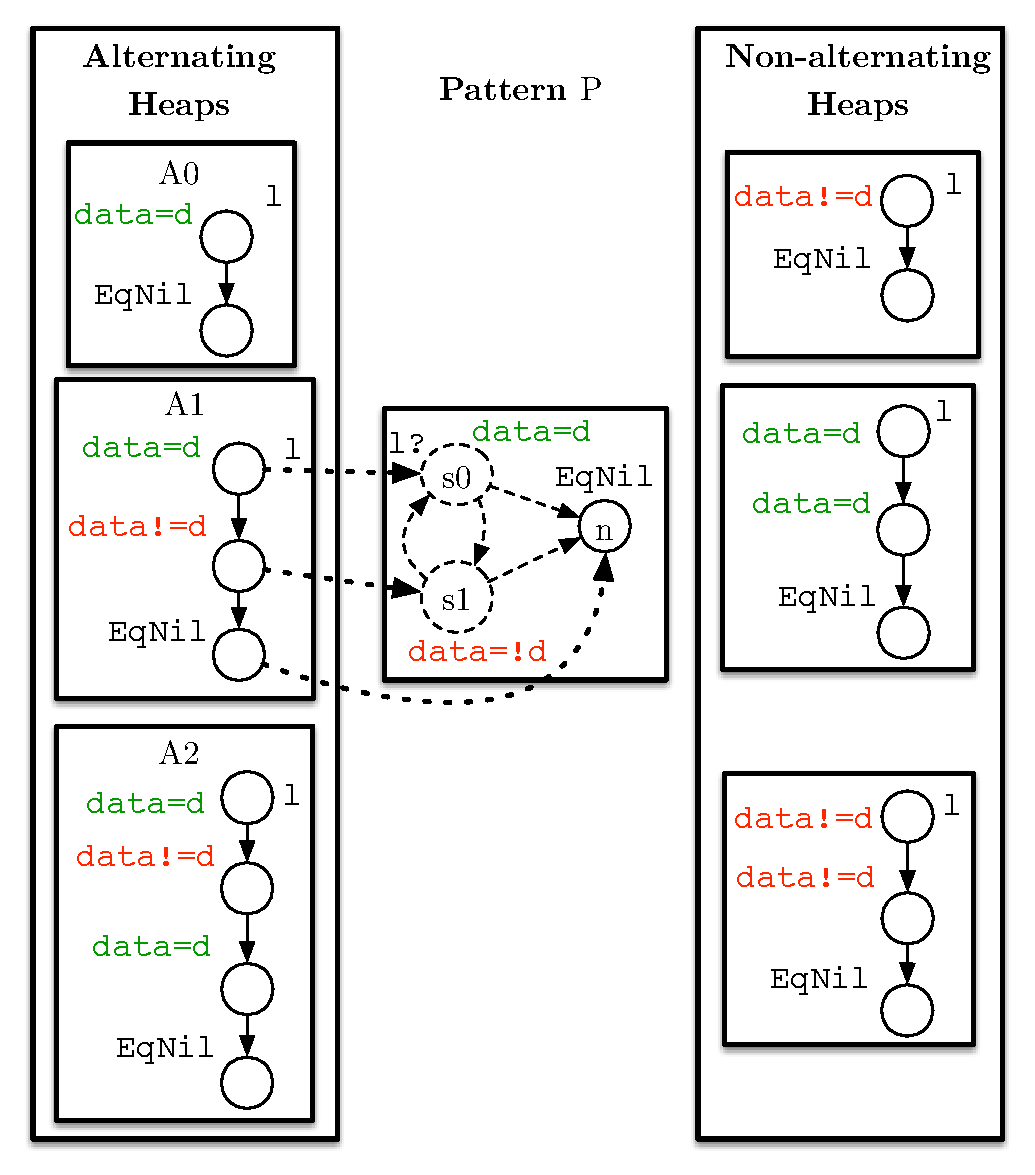
\includegraphics[width=\linewidth]{fig/exs.pdf}
  \caption{Sets of alternating and non-alternating heaps of
    \altlist (\autoref{sec:ex-program}), depicted as graphs, and a
    heap pattern that matches each of the alternating and none
    of the non-alternating heaps.
    %
    The labels of each node $n$ are written adjacent to the node in a heap
    graph are written adjacent to $n$;
    %
    some label values are colored for clarity.
    %
    Each edge is implicitly labeled with the field name \nextnm.
    %
    Each summary node of the pattern $\patnm$ is dashed, each
    indefinite node label is followed by a question mark, and each
    indefinite edge with an indefinite label is dashed.
    %
    The dash-dotted lines from heap $A_1$ to $\patnm$ depict a matching from $A_1$ to $\patnm$.
    %
  }
  \label{fig:alt-pattern}
\end{figure}

% Example: concrete heaps.
\begin{ex}
  \label{ex:concrete-heaps}
  \autoref{fig:alt-pattern} depicts distinct sets of graphs of heaps
  in \altlist states that (1) are alternating and (2) are not
  alternating (for now, ignore the pattern $P$ with dashed nodes and
  edges in the center of \autoref{fig:alt-pattern}).
  %
  The alternating heaps depicted consist of the alternating heaps with
  one to three non-nil cells.
  %
  The non-alternating heaps depicted consist of three non-alternating
  heaps with one to two non-nil cells.
\end{ex}

% Pattern as graph:
Each pattern is a graph in which nodes and edges are labeled from the
space of annotations as the labels on the nodes and edges of heap
graphs.
%
However, a pattern graph may also contain \emph{summary nodes} and
\emph{definite} or \emph{indefinite} labelings. Informally, a definite label indicates a fixed value ($\true$ or $\false$), and an indefinite label indicates that either value is possible.
%
A heap graph $H$ is \emph{matched} by a pattern graph $P$ if there is
a mapping $\matchnm$ from the nodes of $H$ to the nodes of $P$ such
that:
%
\begin{enumerate}
\item
  % Multiple cells only go to a summary node.
  If multiple nodes of $H$ are matched by a node $n$ of $P$, then $n$
  is a summary node.
\item
  % Preserves node labelings.
  For each node $\nodenm$ of $H$, if $\nodenm$ is labeled with label $L$,
  then $\matchnm(\nodenm)$ is either definitely or indefinitely labeled
  with $L$.
  %
  If $\nodenm$ is not labeled with label $L$, then $\matchnm(\nodenm)$
  is either definitely not labeled or indefinitely labeled with $L$.
\item
  % Preserves
  For all nodes $m$ and $n$ of $H$, if there is an edge from $m$ to
  $n$ labeled with field $\fieldnm$, then there is an edge from
  $\matchnm(m)$ to $\matchnm(n)$ either definitely or indefinitely
  labeled with $\fieldnm$.
  %
  If there is no edge from $m$ to $n$ labeled with $\fieldnm$, then
  either there is no edge from $\matchnm(m)$ to $\matchnm(n)$ labeled
  with $\fieldnm$ or there is an edge from $\matchnm(m)$ to
  $\matchnm(n)$ indefinitely labeled with $\fieldnm$.
\end{enumerate}

% Example: walk through the heap graphs and patterns in the example.
\begin{ex}
  \label{ex:heap-pats}
  % Walk through the pattern.
  The heap pattern $\patnm$ depicted in \autoref{fig:alt-pattern}
  matches exactly the alternating heaps of \altlist.
  %
  A matching from the second alternating heap $A_1$ in
  \autoref{fig:alt-pattern} to $\patnm$ is depicted with dotted edges
  from the nodes of the heap to the nodes of the pattern.
  %
  Because $\patnm$ matches each of the alternating heaps and none of
  the non-alternating heaps in \autoref{fig:alt-pattern}, we say that
  $\patnm$ \emph{distinguishes} the alternating and non-alternating
  heaps.
\end{ex}

% Walk through the proof structure for the example.
\section{A proof structure for low-level heap programs}
\label{sec:ex-tree}
% Walk through the example.
\altlist demonstrates that proving that some programs satisfy each of
their assertions, which are defined purely over local variables, may
still sometimes require a verifier to find invariants over the entire
structure of the program heap.
%
In particular, in order to prove that \altlist always satisfies its
assertion at a line 12, a verifier must prove that at line 5, the heap
always holds an alternating list.

% Describe the proof structure in general.
\verifier attempts to construct proofs that are represented as a
partial prefix-tree (i.e., an \emph{unwinding tree}) of the program's
control paths~\cite{mcmillan06}.
% Nodes:
Each node in the tree represents an occurrence of a control location in a
program path, and each edge in the tree represents a step of execution of
the program over a sequence of non-branching instructions.
% Edges.
Each node $n$ is thus identified by a sequence of instructions
$\instrs_n$ that the program must execute to reach the node, and is
annotated with an \emph{invariant}, represented as a heap pattern
(\autoref{sec:ex-patterns}) that is satisfied by all states reached
after the program executes $\instrs_n$.

% Conditions on tree as a valid proof.
A program unwinding $T$ is a proof that a given error location $\errloc$
is unreachable in any run of a program $\mathcal{A}$ if:
%
\begin{enumerate}
%
\item
  % Condition on initial states.
  The initial heap of $\mathcal{A}$ satisfies the invariant at the root of $T$.
\item
  % Adjacent nodes model the semantics of the program.
  For each edge $(m, n)$ in $T$, the invariant at $m$ and the
  semantics of the instructions modeled by the edge $(m, n)$ imply the
  invariant at $n$.
\item
  % Condition on error nodes.
  Each node in $T$ that represents $\errloc$ is annotated with an
  invariant that is not satisfied by any program state.
\item
  % Covering.
  Each leaf $l$ that represents control location $\locnm$ of $T$ either
  represents a terminal control location of $P$, or is \emph{covered} by
  another node of $T$ that represents $\locnm$, and is annotated with a
  weaker invariant than the invariant of $l$.
\end{enumerate}
%
If a leaf $l$ is covered by node $n$, the intuitively the proof tree
need not be further expanded from $l$, because any proof tree rooted
at $n$, which is a proof of safety for all paths with prefix
$\instrs_n$, is a valid proof of safety for all paths with prefix
$\instrs_l$.

% Figure with an annotated unwinding tree.
\begin{figure}
  \centering
  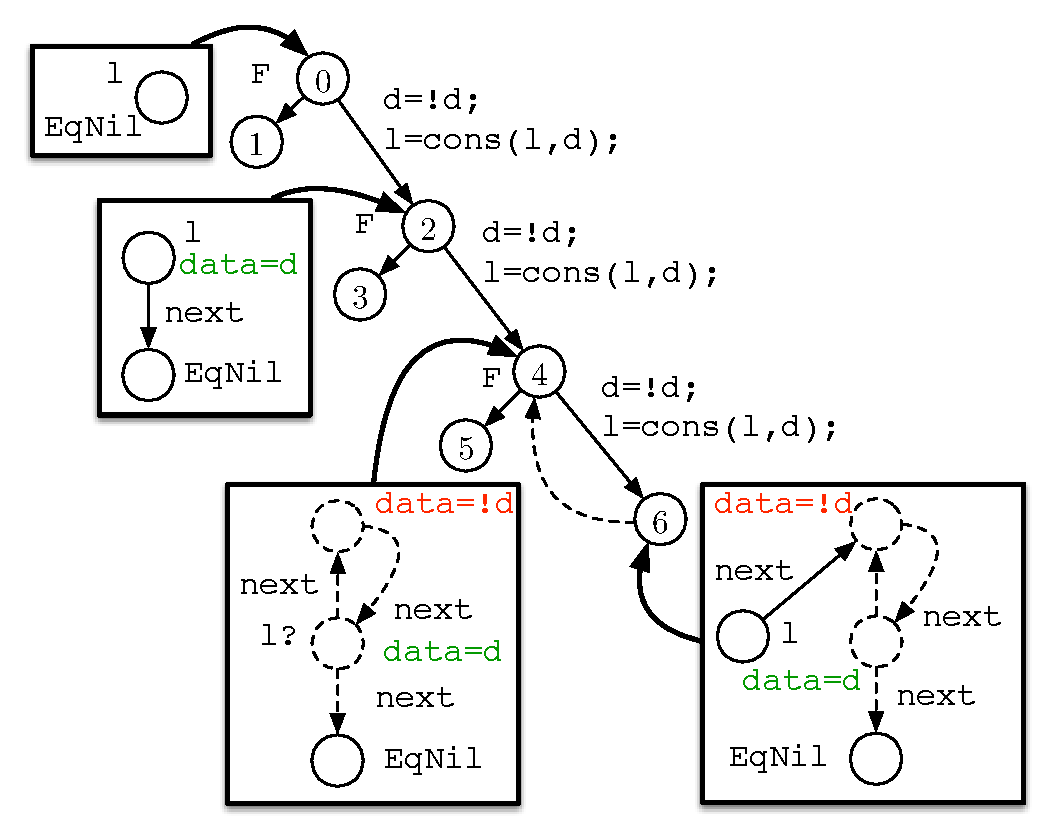
\includegraphics[width=\linewidth]{fig/alt-tree.pdf}
  \caption{The prefix of an unwinding tree $\treenm$ that proves that
    no run of \altlist violates its assertion.
    %
    Edge tree edge is annotated with the instruction sequence that it
    simulates, and each node is annotated with its pattern invariant.
  }
  \label{fig:alt-unwinding}
\end{figure}

% Walk through the unwinding tree for the example program.
\begin{ex}
  \label{ex:alt-list-pf}
  % Give an overview of the example.
  \autoref{fig:alt-unwinding} depicts a prefix tree $T$ of an
  unwinding tree that proves that \altlist always satisfies the
  assertion at line 12.
  %
  $T$ models runs of \altlist that execute \consloop most three times.
  % Talk about nodes.
  Nodes $0$, $2$, $4$, and $6$ model states of \altlist when control
  is at the loop head, and
  %
  nodes $1$, $3$, and $5$ model states of \altlist when control exits
  \consloop.
  % Talk about edges.
  Each edge of $T$ is annotated with the sequence of instructions in
  \altlist that it models.
  %
  Each node $n$ of $T$ is annotated with a heap pattern
  (\autoref{sec:ex-patterns}) that over-approximates the set of heaps
  reachable by executing $\instrs_n$.
  %
  Node $6$ is covered by node $4$ because the pattern at node $6$ is
  entailed by the pattern at node $4$.
  %
  Thus, tree $T$ can be expanded into a complete tree that proves the
  safety of $P$ by expanding $T$ from only leaf nodes $1$, $3$, and
  $5$, not from leaf node $6$.
\end{ex}

% Define heap games.
\section{Learning heap patterns as a game}
\label{sec:ex-heap-games}
% Summary:
The key observation behind the design of \verifier is that any pair of
disjoint sets of heaps $\posheaps$ and $\negheaps$ defines a natural
game, in which the objective for one player is to learn a pattern that
distinguishes $\posheaps$ from $\negheaps$.
% Introduce the key observation: learning is a game.
In particular, let an \emph{inductive pattern synthesizer} be an
Oracle that takes as input a finite set of positive heaps $\posheaps$
and negative heaps $\negheaps$, and returns a heap pattern that is
matched by each heap $\posheaps$ and no heap in $\negheaps$.
%
The synthesizer's goal in the game is to synthesize a heap pattern
that distinguishes $\posheaps$ and $\negheaps$, without direct access
to $\posheaps$ and $\negheaps$.
%
The state of the game consists of finite subsets of \emph{revealed}
$\posheaps_0 \subseteq \posheaps$ and revealed $\negheaps_0 \subseteq
\negheaps$, and a pattern $\patnm$ generated by the synthesizer that
distinguishes $\posheaps_0$ from $\negheaps_0$.
%
In each play, if the inductive pattern synthesizer has not won, then
the pattern verifier reveals either a heap in $\posheaps$ not matched
$\patnm$ or a heap in $\negheaps$ that is matched by $\patnm$.
%
The inductive pattern synthesizer then generates a new pattern that
must match all revealed patterns in $\posheaps$ and no revealed
patterns in $\negheaps$.
% Example: game for line 5.
\begin{ex}
  \label{ex:alt-list-game}
  For \altlist, the reachable heaps and heaps that lead to an
  assertion violation from line $\gamenm_5$ (i.e., the alternating
  heaps and non-alternating heaps) define a pattern-synthesis game
  $\gamenm_5$.
  %
  One valid play of the game with an inductive pattern synthesizer
  $\oraclenm_5$ from a game state consisting of no revealed positive
  heaps and the non-alternating heaps in \autoref{fig:alt-pattern} as
  revealed negative heaps is as follows:
  %
  (1) $\oraclenm_5$ plays the pattern that annotates node $0$ in
  \autoref{fig:alt-unwinding};
  %
  (2) the pattern verifier reveals heap $A_1$ in
  \autoref{fig:alt-pattern};
  %
  (3) $\oraclenm_5$ plays the pattern that annotates node $2$ in
  \autoref{fig:alt-unwinding};
  %
  (4) the pattern verifier reveals heap $A_2$ in
  \autoref{fig:alt-pattern};
  %
  (5) $\oraclenm_5$ plays the pattern that annotates node $4$ in
  \autoref{fig:alt-unwinding} (i.e., pattern $P$ in
  \autoref{fig:alt-pattern}), and wins the game.
\end{ex}

% Walk through how we infer invariants for the example.
\section{From game strategies to program proofs}
\label{sec:ex-infer}
%
The main result of our work is that while the problem of verifying
heap-manipulating programs is undecidable, it can be reduced to
winning a finite set of pattern-synthesis games.
%
The primary difficulty in constructing an unwinding tree $T$ that
proves the safety of a program is in inferring patterns for the nodes
of $T$ that are (1) sufficiently strong enough to prove that each path
of $T$ to an error node is infeasible but (2) sufficiently weak that
they can cover the patterns of sufficiently many leaf nodes to bound
the set of program paths that must be modeled.
%
For the example of \altlist, the pattern on node $4$ of the unwinding
tree in \autoref{fig:alt-unwinding} satisfies both of these criteria;
%
however, in general the problem of inferring sufficient patterns is
undecidable, and to date, there are not general-purpose analyses that
can infer such invariants for practical programs.

% Context: interpolation works for non-graphical data.
In settings where it is not critical to infer properties of the
program's entire heap, it is sufficient to infer invariants for an
unwinding tree by obtaining an \emph{interpolant}~\cite{mcmillan06}
for each node $n$ of two formulas describing (1) states reachable by
executing the instruction sequence of $n$ from the beginning of the
program and (2) states from which $n$ reaches an error.
%
However, interpolation-based approaches must infer interpolants as
formulas in a theory for which the problem of constructing an
interpolant is decidable, typically the combined theory of linear
arithmetic, uninterpreted functions, and arrays (\liufa).
%
Unfortunately, formulas in such theories cannot naturally describe
sets of heaps with arbitrarily many cells, such as the set of
alternating heaps of \altlist (\autoref{sec:ex-program}).

% Our assumption: hypothesis
In this work, we explore a framework in which a verifier can learn heap patterns that are sufficient invariants for proving the correctness of a program, under the assumption that the verifier can query an oracle that can efficiently win a class of the heap-learning games described in \autoref{sec:ex-heap-games}.
%
% Example heaps:
\begin{ex}
  \label{ex:alt-list-pat-syn}
  % Introduce problem:
  Suppose that \verifier has constructed the unwinding tree depicted
  in \autoref{fig:alt-unwinding}, and must choose a pattern with which
  to annotate node $4$, which models line 5 of \altlist.
  %
  \verifier could choose a pattern $P$ that only distinguishes between
  alternating and non-alternating lists of length less than or equal
  to two.
  %
  However, $P$ is, intuitively too strong an invariant in that it
  cannot cover any valid annotation of node $6$.

  % Alternative: choosing patterns as game solutions.
  Alternatively, if \verifier plays the game $\gamenm_5$ as pattern
  verifier against the pattern synthesizer $\oraclenm_5$
  (\autoref{ex:alt-list-game}), and annotates node $4$ with the
  winning pattern played by $\oraclenm_5$ (as depicted in
  \autoref{fig:alt-unwinding}), then \verifier can construct an
  unwinding tree that proves the safety of \altlist.
\end{ex}

% State our main result in formally.
The main result that we present in this thesis is that for a given
program $\prognm$, if our program verifier \verifier has access to an
inductive pattern synthesizer that wins a game defined analogously to
the game $\gamenm_5$ defined for line 5 of \autoref{fig:alt-list}
(\autoref{ex:alt-list-game}) for each control location of $\prognm$,
then \verifier verifies $\prognm$ successfully.

\section*{Summary}
In this chapter, we presented a brief overview of the problem domain, and our approach. Our algorithm extends interpolation-based verification techniques to heap-manipulating programs, using an Oracle to provide input for the interpolation step. The next chapter will focus on technical background for modeling programs for verification.